Para este tema es importante tener claros varios conceptos que vamos a ir definiendo y explicando poco a poco.

\begin{defn}[Middleware]
Conjunto de aplicaciones encargadas de enlazar los componentes de un sistema distribuido.
\end{defn}

\section{Network Operating System (NOS)}
Este conjunto de aplicaciones está dividido en el protocolo específico del servicio con el que estamos trabajando (ODBC, HTTP, SMTP...), el protocolo de transporte (TCP/IP) y una capa intermedia llamada Network Operating System (NOS)}.

\begin{defn}[Network Operating System]
Es una extensión del sistema operativo que proporciona transparencia al cliente, para que éste realice las llamadas como si fueran locales.
\end{defn}

Algunas de las maneras de proporcionar transparencia del NOS según \concept{RM-ODP} (Open Distributed
Processing Reference Model) son
\begin{itemize}
\item Ubicación: Ocultar dónde reside cada recurso (y permite que éste se mueva, incluso mientras está siendo utilizado).
\item Persistencia: Ocultar tanto la activación y desactivación de objetos como sus fallos y recuperaciones mediante la replicación.
\item Concurrencia: Ocultar la utilización de recursos concurrentes.
\item Prestaciones: Escalar el tamaño y reconfigurar el sistema para mejorar sus prestaciones según varía la carga de trabajo.
\item Espacio de nombres:
\item SSO: Single Sign On - Un único usuario y contraseña para todo el sistema.
\item Tiempo: Todos los componentes deben estar sincronizados.
\item Protocolos: Idéntica interfaz de programación para todos los protocolos de transporte.
\end{itemize}

Debido a que la representación interna de los datos es dependiente del ordenador (hardware o sistema operativo) es necesario definir un mecanismo para que, independientemente de la plataforma, la comunicación sea posible. Algunos métodos son utilizar estándares de \textbf{codificación de caracteres} (ISO-8859-1,UTF-8), \textbf{XML}, sistemas propios de aplicaciones (\textbf{RPC,XDR}) o un estándar \textbf{Abstract Synyax Notation} (con una gramática y reglas para codificar los datos).


\section{Servicios de transporte}

Una vez hablado del NOS, vamos a ver unos conceptos de  servicios de transporte del middleware.

Lo primero es recordar que hay 2 modelos de interacción, \textbf{síncrono} o \textbf{asíncrono}. Además de estos modelos, las interacciones pueden ser de tres tipos.
\begin{itemize}
	\item \textbf{R:} Petición. (El cliente hace una petición sin esperar respuesta, por ejemplo para cerrar la conexión)
	\item \textbf{RR:} Petición → Respuesta.
	\item \textbf{RRA:} Petición → Respuesta → ACK.
\end{itemize}

\subsection{API directa}

\begin{defn}[APIs directas]
API viene de \textit{Application Programming Interface} (Interfaz de programación de aplicaciones).

La utilización de APIs directas es la utilización de una interfaz de programación para acceder a unos servicios (proporcionados por la aplicación).
\end{defn}

Habitualmente son servicios de nivel de transporte o sesión. La ubicación de extremos no es transparente para el programa, ya que necesitas saber dónde está la interfaz para poder utilizarla. Para ver un ejemplo de API, consultar: \href{https://apigee.com/OneDrive/embed/console/OneDrive}{API de OneDrive}.

\subsection{Sockets}

Son la leche porque proporcionan mucha transparencia: podemos comunicarnos entre procesos sin tener ni idea de nada, simplemente es como escribir en un fichero (de hecho, si recordamos de Redes II un socket es directamente un descriptor de fichero en Linux).

Aunque ya deberíamos saberlo, incluimos un par de esquemas (sacados de las transparencias) en los que vemos cómo establecer una comunicación orientada a conexión (\ref{SocketConexion}) y una comunicación no orientada a conexión (\ref{SocketNoConexion})


\begin{figure}[hbtp]
\centering
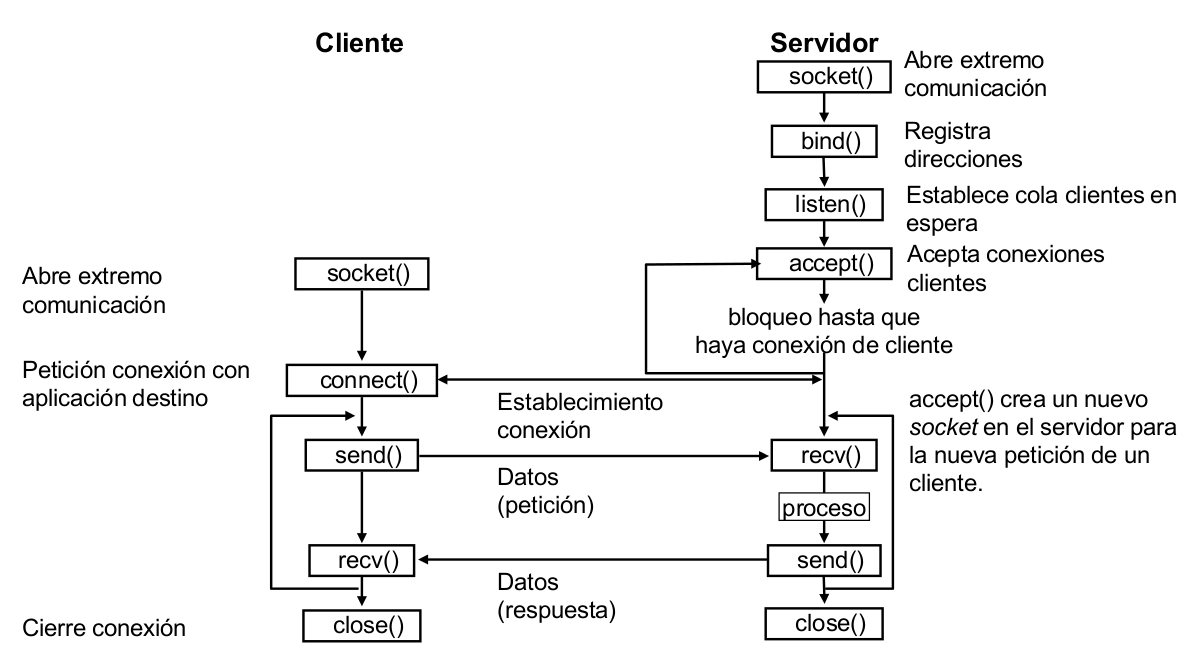
\includegraphics[width=1\textwidth]{img/SocketConexion.png}
\caption{Comunicación orientada a conexión.}
\label{SocketConexion}
\end{figure}

\begin{figure}[hbtp]
\centering
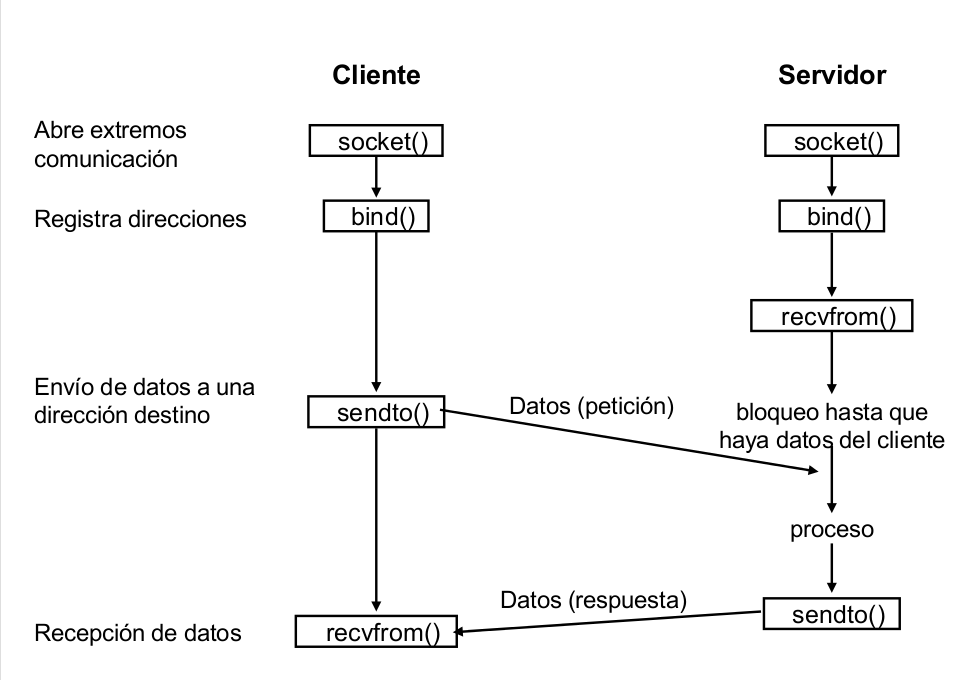
\includegraphics[width=1\textwidth]{img/SocketNoConexion.png}
\caption{Comunicación No Orientada a conexión.}
\label{SocketNoConexion}
\end{figure}
\newpage
\section{Modelos de servicios distribuidos}

La base de este curso es cómo dar servicio a muchos clientes. Si tenemos una web a la que se conectan 10 personas, nos vale con cualquier ordenador, pero ¿Cuánta gente usa google? Ni de coña google tiene un único servidor haciendo todo, tiene que tener los \textbf{servicios distribuidos}. A lo largo de esta sección iremos viendo muchas de las maneras de llevar esto a cabo.

\subsection{RPC - Remote Procedure Calls}
Este modelo se basa en realizar llamadas a funciones como si fueran locales, así el procesamiento de esa función no se realiza en local sino en remoto y nos ahorramos recursos de procesamiento.

Para el funcionamiento de RPCs necesitamos unos componentes intermedios llamados \concept{Stub}. En el siguiente diagrama se entiende perfectamente el funcionamiento de los RPCs.
\begin{figure}[htb]
\centering
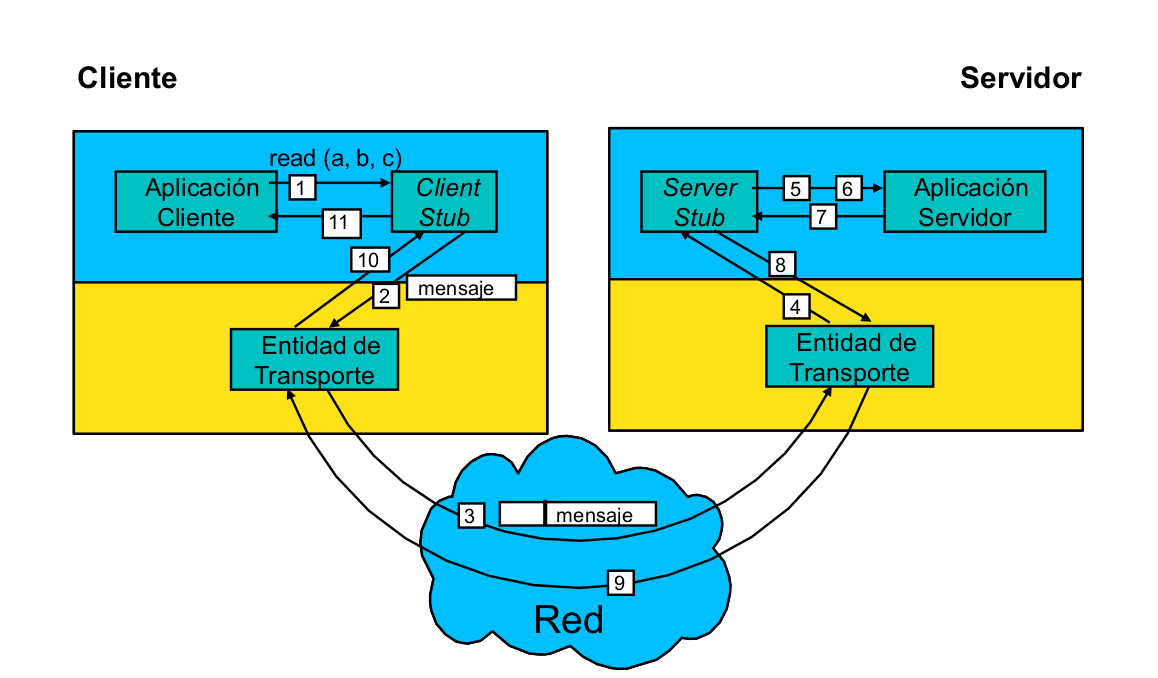
\includegraphics[width=0.9\textwidth]{img/RPC.png}
\caption{Funcionamiento de una llamada RPC.}
\label{RPCimg}
\end{figure}
\newpage

\obs La espera del cliente es \textbf{bloqueante}.

\obs Una ventaja realmente interesante de esto es la transparencia de representación de los datos. RPC (y los stubs intermedios) permiten que un cliente que utiliza Big Endian pueda pasarle los parámetros a una función que se ejecute en un servidor que utiliza Little Endian. Esta \textit{transformación} de los datos de un sistema de codificación al otro se llama \concept{Marshalling} (el codificarlos para enviar) y \concpet{Unmarhsalling} (descodificarlos al recibirlos). Ambos stubs tienen que hacer marshalling y unmarshalling al enviar y recibir mensajes respectivamente.

\paragraph{Problemas de RPC}
\begin{itemize}
	\item No existe el paso de parámetros por referencia.
	\item Hay que conocer de antemano dónde está el servidor exáctamente y en qué puerto escucha.
	\subitem Para saber el puerto en el que el servidor está escuchando, éste tiene que registrarse en un \concept{PortMapper} al que el cliente pregunta por el puerto.
 	\item Tras un \textit{Time Out} No se sabe si la llamada se ha ejecutado o no. Para intentar mitigar este problema en algunos casos, encontramos estrategias distintas en las llamadas RPC:
		\subitem Ejecución Exactamente una vez.
		\subitem Ejecución Como máximo una vez.
		\subitem Ejecución Al menos una vez.\\
	Para solventar esto es necesario también saber si las operaciones son \concept{operaciones de RPC idempotentes} (se pueden ejecutar cualquier número de veces) o no\footnote{Por ejemplo un cálculo $4+4$ lo puedes ejecutar todas las veces que quieras, pero un insert en una base de datos no}.
	\item Es necesaria una representación de datos compartida por los stubs.
	\item Seguridad. ¿Y si el servidor ha sido comprometido y me va a devolver datos que me hagan mal?
\end{itemize}


\paragraph{SUN RPC: } Una de las implementaciones más comunes de RPC es \concept{Sun RPC}. Vamos a estudiarla un poco más en detalle.


Tiene 3 componentes:
\begin{itemize}
	\item \concept{XDR} Lenguaje de definición de tipos de datos. Tiene una sintaxis similar a C, pero es sólo de definición de datos, no de programación
	\item \textbf{Especificación de RPC: } Genera los \textit{stubs} y el fichero de interfaz (para ser incluido al programar)
	\item \textbf{Librería de implementación}
\end{itemize}

Sólo por si interesa, incluimos un esquema de cómo funciona y qué ficheros se generan en la codificación de un servicio utilizando RPC.


\begin{figure}[htb]
\centering
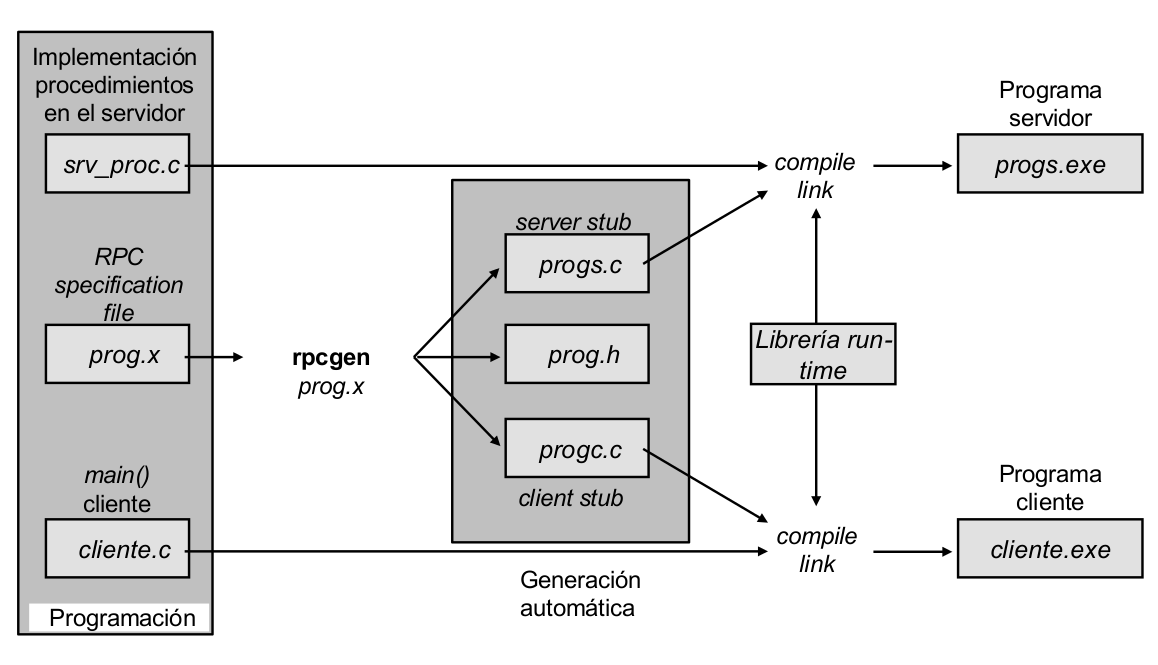
\includegraphics[width=1\textwidth]{img/SUNRPC.png}
\caption{Compilación y generación de código para Sun RPC.}
\label{SunRPC}
\end{figure}

\paragraph{Algunas diferencias entre RPCs}
\begin{itemize}
	\item Parámetros: Aunque en general soporten múltiples parámetros (\concept{Apollo RPC} por ejemplo), Sun RPC sólo tiene un único parámetro, tanto de entrada como de salida (obviamente puedes ser estructuras).
	\item Marshalling: En general lo hace el RPC, aunque en Sun RPC el marshalling que se realiza es mínimo. Es responsabilidad del usuario tener cuidado con eso.
\end{itemize}

Comentamos que Apollo RFC tiene su propio lenguaje de representación de datos, \textit{Network Data Representation} \concept{NDR} (como el XDR de Sun RPC). Apoollo tiene también un lenguaje de representación de interfaces \concept{NIDL} (\textit{Network Interface Definition Language})


\subsection{Web Services (SOAP-WSDL-UDDI)}
Es un modelo de uso de la Web. La idea es tener servidores que ofrecen servicios (localizar geográficamente a través de la IP, ofrecer información de finanzas...) y que cualquiera puede requerir esos servicios. ¿Qué diferencia tiene con RPC? Que en RPC el programador tiene que codificar el lado del servidor y tener conciencia de como funciona, mientras que con los WebServices, el programador que está haciendo un cliente puede utilizar los servicios que le proporciona un servidor que otro programador haya hecho en cualquier otro momento.

Añade un nivel más de transparencia, ya que el programador del cliente no tiene ni idea de cómo funciona el WebService.

La \textbf{función del middleware} aquí es proporcionar funcionalidad para publicar los servicios que ofreces y descubrir los nuevos servicios que vayan surgiendo. Además, tiene que permitir que los servidores soliciten servicios también (multi-\textit{tier}).

\paragraph{Complementos de los Web Services} \concept{OASIS} (Organization for the Advancement of Structured Information Standards) está trabajando (y ha trabajado) en estandarizar una serie de complementos útiles para la mejor utilización de los Web Services y una serie de familia de especificaciones:
\begin{itemize}
\item Complementos:
	\subitem Seguridad.
	\subitem Fiabilidad.
	\subitem Addresing: describir las direcciones de emisor y receptor de un mensaje dentro del propio mensaje.
	\subitem Transaction.
\item \concept{WSRL} - Web Services Resource Framework.
	\subitem WS-Resource (Conjunto de un recurso y un Web Service a través del cual se accede a él.
	\subitem WS-ResourceProperties
	\subitem WS-ResourceLifetime
	\subitem WS-BaseFaults (mecanismo extensible para gestionar errores)
	\subitem WS-ServiceGroup
\end{itemize}

Los WebServices necesitan de 3 protocolos estándares. En el siguiente gráfico se muestran los componentes y protocolos de comunicación utilizados en los WebServices.


\begin{figure}[htb]
\centering
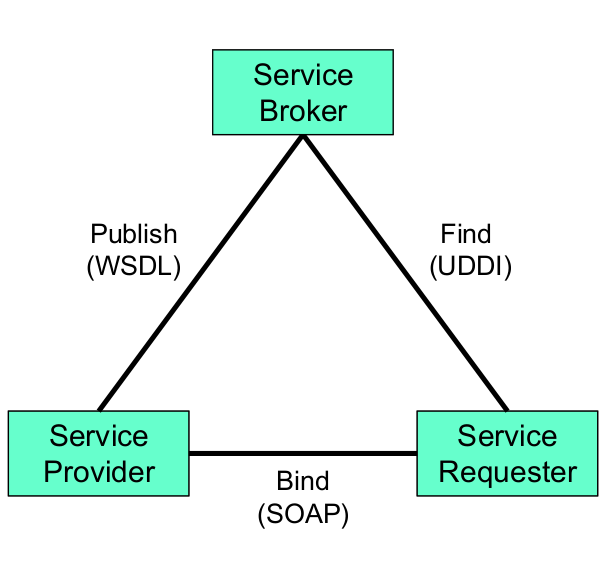
\includegraphics[width=0.9\textwidth]{img/WS.png}
\caption{Componentes de un WS para su funcionamiento.}
\label{WSimg}
\end{figure}


\subsubsection{SOAP}
\subsubsection{WSDL}
\subsubsection{UDDI}

\paragraph{Ventajas e inconvenientes}

\subsection{Rest}

\subsection{Comuncación mediante colas de mensajes}

\begin{defn}[MOM]
Message Oriented Middleware.

Es un proceso asíncrono en el que se genera un mensaje, se encola y se sigue lo que se estaba. Como mandar un correo electrónico, que se encola en la bandeja de entrada y tu sigues trabajando.
\end{defn}

Las conexiones en colas de mensajes pueden ser 1-1, 1-N, N-1 y N-M.

\paragraph{Situaciones ideales}
\begin{itemize}
 	\item Conexiones no permanentes y costosas.
 	\item Múltiples servidores procesando mensajes de clientes.
 	\item Llegada de mensajes impredecibles o en ráfagas
 	\item Sistemas de tipo publicación/suscripción.
 \end{itemize}
 \obs Permite balanceo automático de carga en un sistema distribuido. Se pueden procesar los mensajes con prioridades, no necesariamente FIFO.

Vamos a ver algunos ejemplos de gestores de colas.
\subsubsecction{IBM Web Sphere MQ}
Es el MOM más extendido. Es multiplataforma y multiprotocolo.


\concept{IBM Sphere MQ} está formado por
\begin{itemize}
	\item Gestores de colas, encargados de manejar el envío y recepción de los mensajes, además de crear y gestionar el resto de los elementos.

	Tiene una API con
	\subitem Message Queuing Interface (MQI)
	\subitem Application Messagin Interface (AMI)
	\subitem Java Messaging Services (JMS)
	\item Colas de mensajes de múltiples tipos.
	\item Canales de comunicación: Conexiones unidireccionales entre gestores de colas.
\end{itemize}

A continuación mostramos un esquema de funcionamiento de un sistema de mensajería de colas:


\begin{figure}[hbtp]
\centering
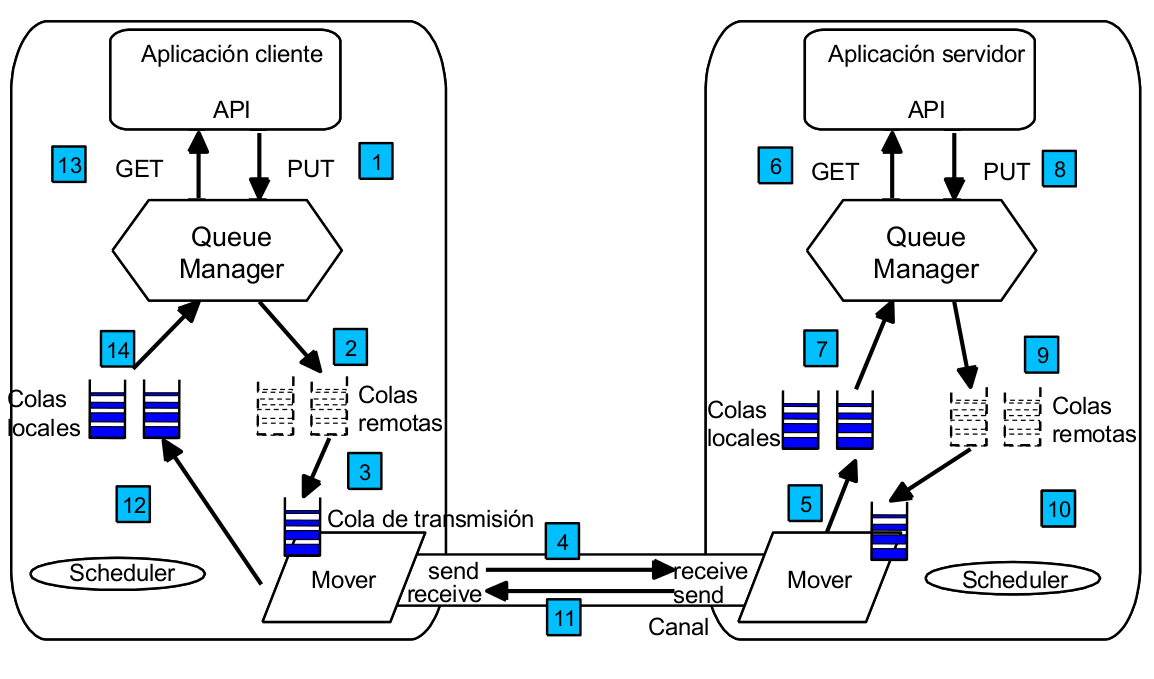
\includegraphics[width=1\textwidth]{img/MOMGen.png}
\caption{Sistema de mensajería de colas.}
\label{MOMGen}
\end{figure}
\newpage

Vemos que se distinguen 3 tipos de colas, las locales (del propio sistema) y las remotas, que el sistema reconoce que pertenecen a otro sistema y entonces el mensaje tiene que ser enviado al sistema al que pertenece la cola remota.

Además de estos 3 tipos de colas (locales remotas y de transmisión) podemos definir en nuestras colas un par de propiedades: persistentes o temporales (en el almacenamiento de los mensajes) y estáticas (definidas permanentemente) o dinámicas (creadas por aplicaciones). Las colas dinámicas se crean a partir de una cola modelo.

También existen las colas de activación, y de cartas muertas (con mensajes que no se han podido entregar)


En resumen, los tipos de colas pueden ser:
\begin{itemize}
	\item Local - remota.
	\item Persistente - temporal.
	\item Estática - dinámica.
	\item Activación.
	\item Cartas muertas.
	\item Transmisión.
\end{itemize}

\begin{example}
Una de las utilidades de MOM son los servicios de publicación/suscripción. A continuación incluimos un esquema que muestra perfectamente cómo funcionan este tipo de sistemas.


\begin{figure}[hbtp]
\centering
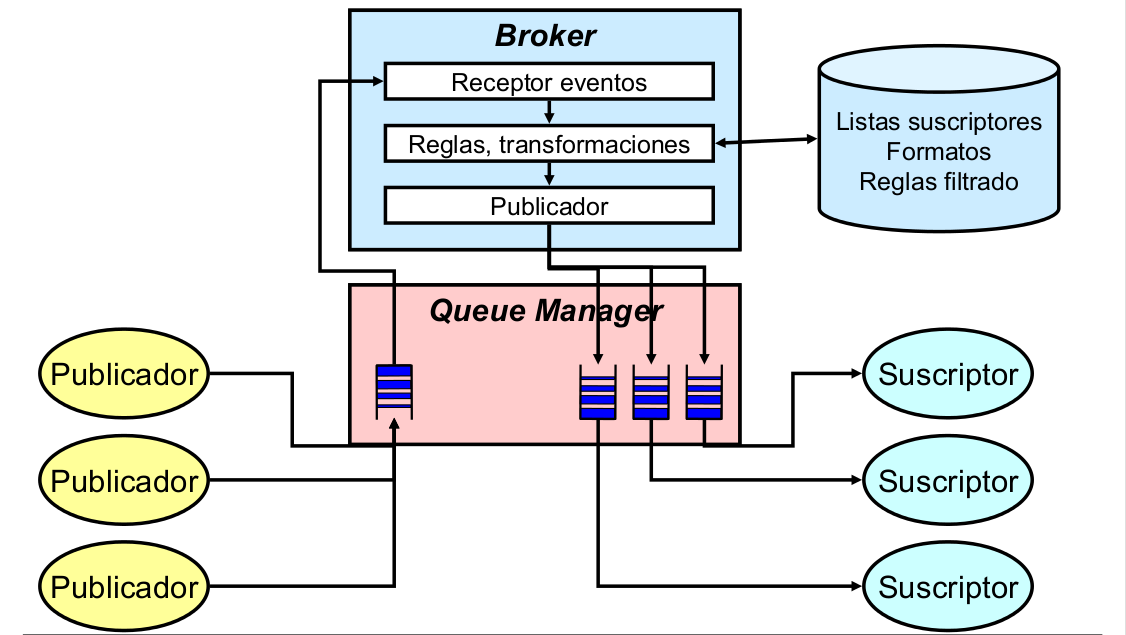
\includegraphics[width=1\textwidth]{img/PubSusc.png}
\caption{Sistema publicador/suscriptor.}
\label{PubSusc}
\end{figure}
\newpage
\end{example}


\section{Services Oriented Architecture SOA}
\subsection{ESB - Enterprise Services Bus}

Extendiendo el modelo de publicador/suscriptor tenemos un ESB. El ESB actúa como proceso centralizador de solicitudes de los clientes (normalmente mensajes o solicitudes de ejecución de acciones tipo RPC – Web Services) para su distribución a los servidores.


\begin{figure}[hbtp]
\centering
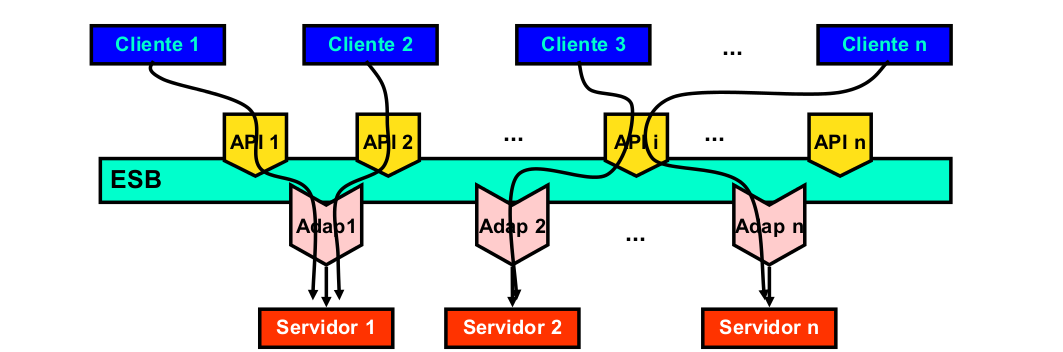
\includegraphics[width=1\textwidth]{img/ESB.png}
\caption{Enterprise Service Bus.}
\label{ESB}
\end{figure}

A continuación, estudiamos las ventajas e inconvenientes que puede tener un sistema como este:
\paragrpaph{Ventajas:}
\begin{itemize}
\item Adaptación rápida en entornos existentes.
\item Flexibilidad. Fácil de adaptar a nuevos requerimientos.
\item Basado en estándares.
\item Existencia de tipos de servicios y APIs predefinidas y listas para su uso.
\item Convierte tareas de programación en configuración (manipulación de datos, por ejemplo).
\item Facilita la gestionabilidad del sistema, al proporcionar un punto único de control para todos los intercambios.
\end{itemize}
\paragrpaph{ Inconvenientes:}
\begin{itemize}
\item Posible punto único de fallo.
\item Fácil saturación del ESB a cargas altas de comunicación.
\item Sin una planificación correcta de APIs y conectores no evita la conexión lógica punto a punto entre clientes y servidores, sólo la física.
\item Requiere más sistemas en ejecución, para soportar el propio ESB.
\item Introducción de un elemento adicional en la cadena de procesamiento, con lo cual el rendimiento se puede ver afectado.
\item Escasas ventajas para entornos sencillos. Estas se ven más en situaciones complejas, con muchos tipos de clientes y servidores.
\end{itemize}

\subsection{RMI - Remote Method Invocation}

Igual que en programación estructurada podíamos ejecutar funciones remotamente (con RPC), con la programación orientada a objetos (POO) también podemos tener localmente una referencia a un objeto remoto y ejecutar métodos del objeto remoto. Para ello es necesario disponer de un middleware espefícico, con unos módulos de comunicación y de referencia remota.


\begin{figure}[hbtp]
\centering
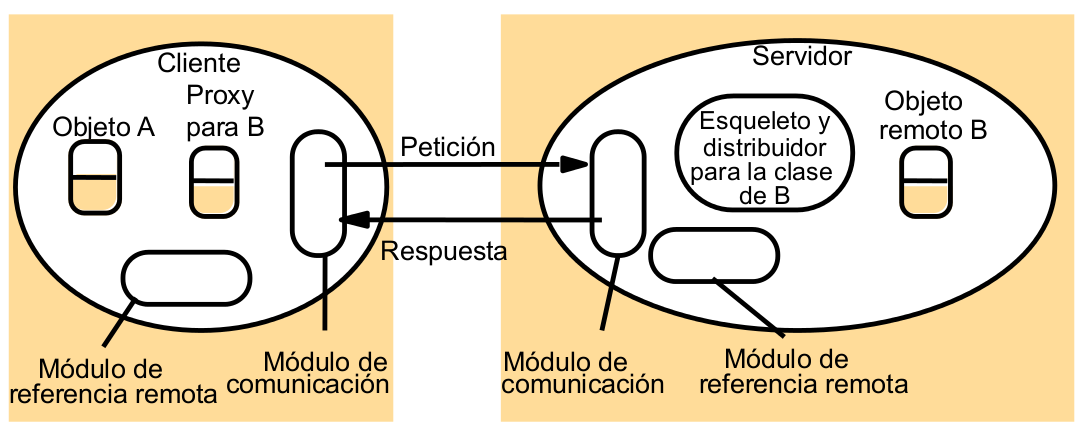
\includegraphics[width=1\textwidth]{img/RMI.png}
\caption{Esquema de funcionamiento de RMI.}
\label{RMI}
\end{figure}

En RMI también es necesario realizar marshalling y unmarshalling. El componente encargado de hacerlo es el esqueleto (del objeto remoto).

El otro componente que merece mención es el módulo de la referencia remota. El objeto que tiene el cliente es una referencia que el módulo de referencias remotas se encarga de traducir la referencia local (a algo remoto) a una referencia remota (al objeto remoto).

Aparte del RMI de Java, existen otras alternativas, como \concept{CORBA} (Common Object Request Broker Architecture) creada por \concept{OMG} (Object Management Group) y \concpet{DCOM} (Distributed Component Object Model) creada por Microsoft.

\subsubsection{OMA}
\begin{defn}[OMA]
Object Management Architecture.

Establece 2 modelos. Un modelo de objetos y uno de referencias.
\end{defn}

Vamos a ver el modelo de referencias.


\begin{figure}[hbtp]
\centering
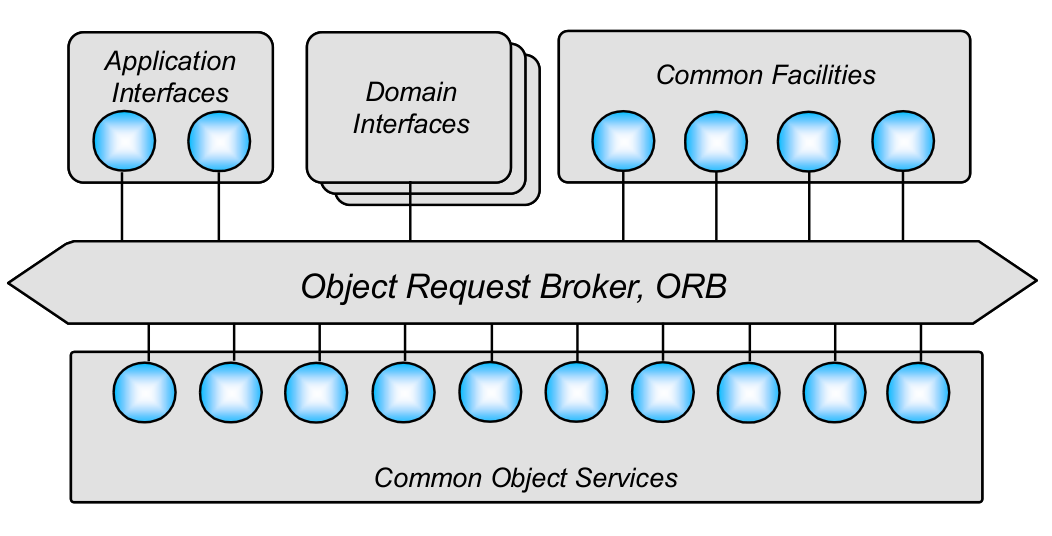
\includegraphics[width=1\textwidth]{img/OMA_Ref.png}
\caption{Esquema de funcionamiento del modelo de referencias de OMA.}
\label{OMA}
\end{figure}

\begin{itemize}
	\item \textit{Object Request Broker, ORB:} Bus de comunicación entre objetos.
	\item \textit{Common Object Services:} Gestión del ciclo de vida, persistencia, resolución de nombres, tiempo, control de concurrencia, seguridad...
	\item \textit{Common Facilities:} Colecciones de componentes, con funciones de tipo general, pero orientados a aplicaciones finales en vez de al sistema.
	\item \textit{Domain Interfaces:} Colección de componentes/objetos comunes específicos para áreas de aplicaciones: comercio electrónico, telecomunicaciones, banca, salud, fabricación...
	\item \textit{Application Interfaces:} Interfaces específicas de aplicaciones concretas.
\end{itemize}

\begin{defn}[ORB]
Object Request Broker → Bus de comunicación entre objetos.

Es un middleware avanzado que es la repera y permite :

\begin{itemize}
	\item Permite llamadas estáticas y dinámicas a objetos. Incluye descubrimiento dinámico de objetos.
	\item Describir las interfaces independientemente del lenguaje de programación. El lenguaje de descripción se llama IDL (Interface Description Language)
	\item Enlace directo de aplicaciones escritas en múltiples lenguajes de alto nivel (no necesariamente orientados a objetos).
	\item Sistema auto-descrito. Genera meta-información consultable dinámicamente.
	\item Soporte de seguridad,transacciones y autenticación de las comunicaciones
	\item Polimorfismo en la ejecución de funciones asociadas a un mismo mensaje.
\end{itemize}
\end{defn}

\begin{defn}[IDL]
Interface description language.
\end{defn}

Del código IDL se crean los stubs necesarios (cliente y servidor\footnote{Los stubs de servidor se llaman \textit{skeletons}}) y los ficheros de definiciones. Además, se genera código fuente del lenguaje elegido, definido en CORBA.

Este es el esquema de desarrollo de un sistema con CORBA.


\begin{figure}[hbtp]
\centering
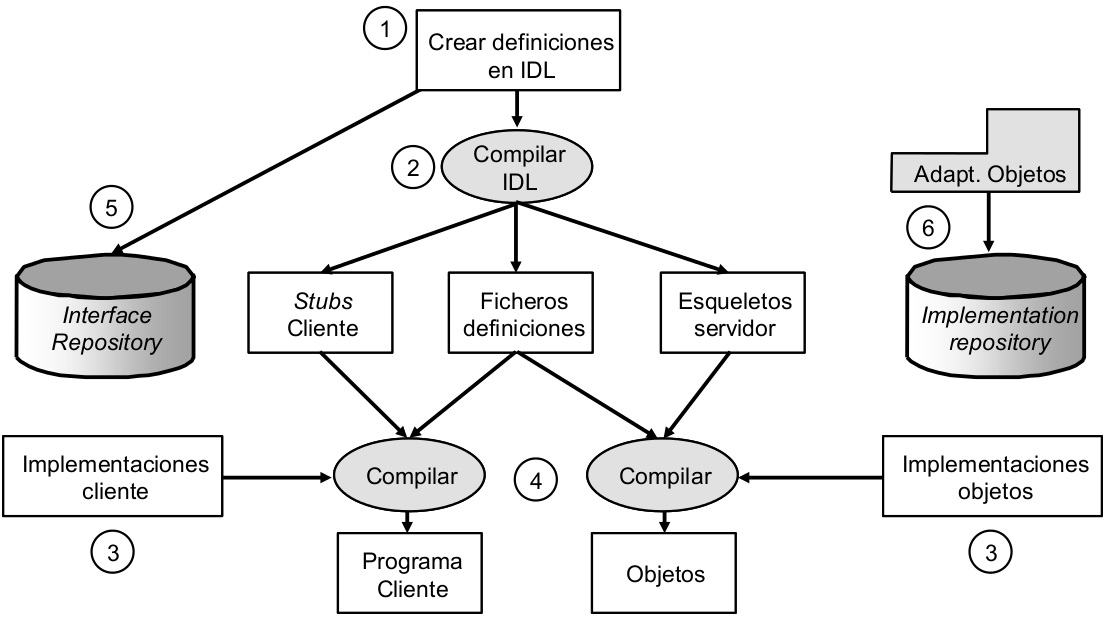
\includegraphics[width=1\textwidth]{img/CORBA.png}
\caption{Esquema del desarrollo de CORBA.}
\label{OMA}
\end{figure}

\subsubsection{DCOM}
